%%__________________________________________________________________||
\section{Results and interpretation}
\label{sec:interpretation}

A likelihood model of the observations in all data samples is
used to obtain a consistent prediction of the SM backgrounds and to
test for the presence of a variety of signal models.

In each bin of \scalht, the observation is modelled as a
Poisson-distributed variable around the sum of the SM expectation and a
potential signal contribution (assumed to be zero in the following
discussion). The SM expectation is related to the expected yields in
the \mj, \mmj, and \gj control samples via the transfer factors
derived from simulation. Likelihood functions describe the yields in the \scalht bins
of the \mj, \mmj, and \gj control samples in the same category of
\njet and \nb as the signal region. The systematic uncertainties
associated with the transfer factors are accommodated in the
likelihood function by a nuisance parameter per transfer factor. The
measurements of these parameters are assumed to follow a log-normal
distribution. The CL$_{\mathrm{s}}$ technique~\cite{read, Cowan:2010js} was used to set limits using asymptotic formulae.

The expected number of events from SM processes is determined from a
simultaneous fit to the signal region and up to three control
samples. The likelihood function is maximised over all fit parameters
under the SM-only hypothesis.
Tables~\ref{tab:yieldsewkdatapost_sig_comb_sym} and \ref{tab:yieldsewkdatapost_sig_comb_asym} and
\ref{tab:yieldsewkdatapost_sig_comb_mono} summarise
the observed yields and fit results with associated errors in bins of \scalht for events in the signal region
categorised according to \njet and \nb. 
No significant tension is observed between the predictions and data in the
signal region which is well described by the SM-only hypothesis.

\begin{table}[h!]
\tiny
\centering
\caption{Predictions and Data in the signal region for 1.26\ifb for symmetric categories. The letter ``a'' in jet \eg ``2a''  indicates the asymmetric jet bins. All entries are non-zero but are truncated to one decimal place.\label{tab:yieldsewkdatapost_sig_comb_sym}}
\begin{tabular}
{cccccccccc}
	\hline\hline
&	&	& \multicolumn{8}{c}{\scalht (\gev)}\\ 
	&	 (\njet, \nb) & 200-250 & 250-300 & 300-350 & 350-400 & 400-500 & 500-600 & 600-800 & 800-$\infty$ \\ [0.8ex] 
\hline
	SM & (2, 0) & $559.6^{+ 25.3 }_{- 25.3 }$ & $599.0^{+ 27.4 }_{- 27.4 }$ & $398.0^{+ 19.7 }_{- 19.7 }$ & $246.9^{+ 18.0 }_{- 18.0 }$ & $196.5^{+ 12.9 }_{- 12.9 }$ & $53.6^{+ 7.4 }_{- 7.4 }$ & $36.8^{+ 5.6 }_{- 5.6 }$ & $30.7^{+ 4.8 }_{- 4.8 }$ \\[0.5ex] 
	Data & (2, 0) & 552 & 592 & 395 & 247 & 189 & 55 & 39 & 33 \\[0.5ex] 
	SM & (2, 1) & $73.7^{+ 7.0 }_{- 7.0 }$ & $57.2^{+ 6.2 }_{- 6.2 }$ & $32.7^{+ 4.6 }_{- 4.6 }$ & $22.0^{+ 4.0 }_{- 4.0 }$ & $16.5^{+ 2.4 }_{- 2.4 }$ & $4.1^{+ 1.3 }_{- 1.3 }$ & $2.9^{+ 1.0 }_{- 1.0 }$ & $3.2^{+ 0.9 }_{- 0.9 }$ \\[0.5ex] 
	Data & (2, 1) & 81 & 63 & 35 & 22 & 23 & 3 & 1 & 2 \\[0.5ex] 
	SM & (2, 2) & $1.6^{+ 1.2 }_{- 1.2 }$ & $1.8^{+ 1.3 }_{- 1.3 }$ & $1.2^{+ 0.8 }_{- 0.8 }$ & -- & $1.0^{+ 0.4 }_{- 0.4 }$ & $0.3^{+ 0.3 }_{- 0.3 }$ & $0.2^{+ 0.2 }_{- 0.2 }$ & $0.1^{+ 0.2 }_{- 0.2 }$ \\[0.5ex] 
	Data & (2, 2) & 2 & 3 & 2 & -- & 2 & 0 & 0 & 0 \\[0.5ex] 
	SM & (3, 0) & $1.4^{+ 1.9 }_{- 1.9 }$ & $111.2^{+ 10.7 }_{- 10.7 }$ & $282.0^{+ 16.7 }_{- 16.7 }$ & $280.0^{+ 16.0 }_{- 16.0 }$ & $348.4^{+ 20.3 }_{- 20.3 }$ & $121.4^{+ 9.7 }_{- 9.7 }$ & $53.1^{+ 6.3 }_{- 6.3 }$ & $46.1^{+ 4.6 }_{- 4.6 }$ \\[0.5ex] 
	Data & (3, 0) & 1 & 111 & 283 & 282 & 353 & 120 & 51 & 51 \\[0.5ex] 
	SM & (3, 1) & $1.4^{+ 1.4 }_{- 1.4 }$ & $24.3^{+ 4.0 }_{- 4.0 }$ & $45.0^{+ 5.0 }_{- 5.0 }$ & $57.1^{+ 6.0 }_{- 6.0 }$ & $42.5^{+ 6.0 }_{- 6.0 }$ & $15.3^{+ 2.5 }_{- 2.5 }$ & $9.0^{+ 2.1 }_{- 2.1 }$ & $5.5^{+ 1.1 }_{- 1.1 }$ \\[0.5ex] 
	Data & (3, 1) & 2 & 25 & 49 & 60 & 35 & 16 & 10 & 5 \\[0.5ex] 
	SM & (3, 2) & -- & $4.4^{+ 1.2 }_{- 1.2 }$ & $9.0^{+ 1.9 }_{- 1.9 }$ & $8.2^{+ 1.7 }_{- 1.7 }$ & $6.8^{+ 1.4 }_{- 1.4 }$ & $2.1^{+ 0.6 }_{- 0.6 }$ & $0.9^{+ 0.3 }_{- 0.3 }$ & $0.2^{+ 0.2 }_{- 0.2 }$ \\[0.5ex] 
	Data & (3, 2) & -- & 4 & 4 & 4 & 9 & 3 & 2 & 0 \\[0.5ex] 
	SM & (3, $\ge3$) & -- & -- & -- & $0.7^{+ 0.8 }_{- 0.8 }$ & $0.2^{+ 0.2 }_{- 0.2 }$ & $0.1^{+ 0.1 }_{- 0.1 }$ & -- & -- \\[0.5ex] 
	Data & (3, $\ge3$) & -- & -- & -- & 0 & 1 & 0 & -- & -- \\[0.5ex] 
	SM & (4, 0) & -- & -- & $30.5^{+ 5.7 }_{- 5.7 }$ & $95.1^{+ 9.7 }_{- 9.7 }$ & $167.5^{+ 11.0 }_{- 11.0 }$ & $91.4^{+ 9.8 }_{- 9.8 }$ & $60.7^{+ 7.8 }_{- 7.8 }$ & $31.4^{+ 3.7 }_{- 3.7 }$ \\[0.5ex] 
	Data & (4, 0) & -- & -- & 31 & 93 & 158 & 92 & 60 & 33 \\[0.5ex] 
	SM & (4, 1) & -- & -- & $9.7^{+ 3.1 }_{- 3.1 }$ & $43.5^{+ 6.0 }_{- 6.0 }$ & $58.2^{+ 5.9 }_{- 5.9 }$ & $16.8^{+ 3.4 }_{- 3.4 }$ & $10.9^{+ 2.2 }_{- 2.2 }$ & $7.3^{+ 1.0 }_{- 1.0 }$ \\[0.5ex] 
	Data & (4, 1) & -- & -- & 7 & 44 & 64 & 14 & 10 & 5 \\[0.5ex] 
	SM & (4, 2) & -- & -- & $2.8^{+ 1.4 }_{- 1.4 }$ & $15.0^{+ 3.0 }_{- 3.0 }$ & $19.2^{+ 2.7 }_{- 2.7 }$ & $4.5^{+ 1.2 }_{- 1.2 }$ & $2.3^{+ 0.6 }_{- 0.6 }$ & $1.4^{+ 0.3 }_{- 0.3 }$ \\[0.5ex] 
	Data & (4, 2) & -- & -- & 5 & 15 & 24 & 7 & 4 & 0 \\[0.5ex] 
	SM & (4, $\ge3$) & -- & -- & -- & $1.4^{+ 0.9 }_{- 0.9 }$ & $1.1^{+ 0.7 }_{- 0.7 }$ & $0.4^{+ 0.3 }_{- 0.3 }$ & $0.1^{+ 0.1 }_{- 0.1 }$ & $0.0^{+ 0.0 }_{- 0.0 }$ \\[0.5ex] 
	Data & (4, $\ge3$) & -- & -- & -- & 3 & 0 & 0 & 0 & 0 \\[0.5ex] 
	SM & ($\ge5$, 0) & -- & -- & -- & $4.0^{+ 2.0 }_{- 2.0 }$ & $54.1^{+ 6.8 }_{- 6.8 }$ & $45.4^{+ 6.6 }_{- 6.6 }$ & $41.8^{+ 5.6 }_{- 5.6 }$ & $31.6^{+ 3.8 }_{- 3.8 }$ \\[0.5ex] 
	Data & ($\ge5$, 0) & -- & -- & -- & 5 & 55 & 47 & 41 & 36 \\[0.5ex] 
	SM & ($\ge5$, 1) & -- & -- & -- & $1.3^{+ 0.9 }_{- 0.9 }$ & $31.4^{+ 4.5 }_{- 4.5 }$ & $18.1^{+ 3.1 }_{- 3.1 }$ & $14.9^{+ 3.0 }_{- 3.0 }$ & $10.9^{+ 1.8 }_{- 1.8 }$ \\[0.5ex] 
	Data & ($\ge5$, 1) & -- & -- & -- & 1 & 34 & 17 & 16 & 13 \\[0.5ex] 
	SM & ($\ge5$, 2) & -- & -- & -- & $0.8^{+ 0.6 }_{- 0.6 }$ & $11.7^{+ 2.5 }_{- 2.5 }$ & $9.0^{+ 1.9 }_{- 1.9 }$ & $4.6^{+ 1.2 }_{- 1.2 }$ & $2.7^{+ 0.6 }_{- 0.6 }$ \\[0.5ex] 
	Data & ($\ge5$, 2) & -- & -- & -- & 0 & 9 & 9 & 5 & 4 \\[0.5ex] 
	SM & ($\ge5$, $\ge3$) & -- & -- & -- & -- & $0.9^{+ 0.5 }_{- 0.5 }$ & $0.4^{+ 0.3 }_{- 0.3 }$ & $0.7^{+ 0.4 }_{- 0.4 }$ & $0.3^{+ 0.1 }_{- 0.1 }$ \\[0.5ex] 
	Data & ($\ge5$, $\ge3$) & -- & -- & -- & -- & 0 & 0 & 0 & 3 \\[0.5ex] 
	\hline
	\hline
\end{tabular}
\end{table}

\begin{table}[h!]
\tiny
\centering
\caption{Predictions and Data in the signal region for 1.26\ifb for asymmetric categories. The letter ``a'' in jet \eg ``2a''  indicates the asymmetric jet bins. All entries are non-zero but are truncated to one decimal place.\label{tab:yieldsewkdatapost_sig_comb_asym}}
\begin{tabular}
{cccccccccc}
	\hline\hline
&	&	& \multicolumn{8}{c}{\scalht (\gev)}\\ 
	&	 (\njet, \nb) & 200-250 & 250-300 & 300-350 & 350-400 & 400-500 & 500-600 & 600-800 & 800-$\infty$ \\ [0.8ex] 
\hline
	SM & (2a, 0) & $2894.8^{+ 53.6 }_{- 53.6 }$ & $854.8^{+ 28.8 }_{- 28.8 }$ & $293.3^{+ 16.3 }_{- 16.3 }$ & $141.9^{+ 11.4 }_{- 11.4 }$ & $83.3^{+ 9.1 }_{- 9.1 }$ & $11.3^{+ 3.3 }_{- 3.3 }$ & $7.7^{+ 3.1 }_{- 3.1 }$ & -- \\[0.5ex] 
	Data & (2a, 0) & 2887 & 857 & 290 & 143 & 83 & 11 & 8 & -- \\[0.5ex] 
	SM & (2a, 1) & $246.7^{+ 12.6 }_{- 12.6 }$ & $81.7^{+ 6.3 }_{- 6.3 }$ & $25.2^{+ 3.3 }_{- 3.3 }$ & $12.4^{+ 2.5 }_{- 2.5 }$ & $6.1^{+ 1.3 }_{- 1.3 }$ & $0.9^{+ 0.5 }_{- 0.5 }$ & $0.3^{+ 0.4 }_{- 0.4 }$ & -- \\[0.5ex] 
	Data & (2a, 1) & 254 & 77 & 29 & 12 & 7 & 1 & 0 & -- \\[0.5ex] 
	SM & (2a, 2) & $14.5^{+ 2.5 }_{- 2.5 }$ & $3.5^{+ 0.9 }_{- 0.9 }$ & $2.5^{+ 0.9 }_{- 0.9 }$ & $1.7^{+ 0.7 }_{- 0.7 }$ & $0.6^{+ 0.3 }_{- 0.3 }$ & $0.0^{+ 0.3 }_{- 0.3 }$ & $0.1^{+ 0.2 }_{- 0.2 }$ & -- \\[0.5ex] 
	Data & (2a, 2) & 15 & 6 & 2 & 1 & 0 & 0 & 0 & -- \\[0.5ex] 
	SM & (3a, 0) & $743.4^{+ 26.9 }_{- 26.9 }$ & $792.7^{+ 27.2 }_{- 27.2 }$ & $374.0^{+ 19.0 }_{- 19.0 }$ & $125.3^{+ 10.4 }_{- 10.4 }$ & $52.9^{+ 6.9 }_{- 6.9 }$ & $10.0^{+ 3.5 }_{- 3.5 }$ & $3.4^{+ 2.0 }_{- 2.0 }$ & -- \\[0.5ex] 
	Data & (3a, 0) & 739 & 798 & 372 & 118 & 55 & 11 & 3 & -- \\[0.5ex] 
	SM & (3a, 1) & $148.4^{+ 10.7 }_{- 10.7 }$ & $143.4^{+ 9.8 }_{- 9.8 }$ & $62.6^{+ 7.1 }_{- 7.1 }$ & $27.0^{+ 4.7 }_{- 4.7 }$ & $6.3^{+ 1.6 }_{- 1.6 }$ & $0.9^{+ 0.6 }_{- 0.6 }$ & $0.7^{+ 0.8 }_{- 0.8 }$ & -- \\[0.5ex] 
	Data & (3a, 1) & 152 & 135 & 66 & 35 & 5 & 0 & 1 & -- \\[0.5ex] 
	SM & (3a, 2) & $25.7^{+ 3.5 }_{- 3.5 }$ & $25.0^{+ 2.9 }_{- 2.9 }$ & $13.9^{+ 2.4 }_{- 2.4 }$ & $5.7^{+ 1.6 }_{- 1.6 }$ & $0.9^{+ 0.4 }_{- 0.4 }$ & $0.2^{+ 0.2 }_{- 0.2 }$ & $0.0^{+ 0.1 }_{- 0.1 }$ & -- \\[0.5ex] 
	Data & (3a, 2) & 25 & 28 & 12 & 5 & 0 & 0 & 0 & -- \\[0.5ex] 
	SM & (3a, $\ge3$) & $0.5^{+ 0.3 }_{- 0.3 }$ & $0.8^{+ 0.4 }_{- 0.4 }$ & $0.5^{+ 0.4 }_{- 0.4 }$ & -- & $0.0^{+ 0.0 }_{- 0.0 }$ & -- & -- & -- \\[0.5ex] 
	Data & (3a, $\ge3$) & 2 & 1 & 1 & -- & 0 & -- & -- & -- \\[0.5ex] 
	SM & (4a, 0) & $0.7^{+ 1.1 }_{- 1.1 }$ & $70.3^{+ 10.0 }_{- 10.0 }$ & $183.2^{+ 12.4 }_{- 12.4 }$ & $105.1^{+ 9.2 }_{- 9.2 }$ & $57.7^{+ 7.3 }_{- 7.3 }$ & $5.5^{+ 2.4 }_{- 2.4 }$ & $1.6^{+ 1.7 }_{- 1.7 }$ & -- \\[0.5ex] 
	Data & (4a, 0) & 0 & 68 & 182 & 102 & 58 & 5 & 2 & -- \\[0.5ex] 
	SM & (4a, 1) & $0.3^{+ 0.7 }_{- 0.7 }$ & $23.6^{+ 4.8 }_{- 4.8 }$ & $74.6^{+ 7.2 }_{- 7.2 }$ & $46.3^{+ 5.7 }_{- 5.7 }$ & $27.7^{+ 4.6 }_{- 4.6 }$ & $1.3^{+ 0.7 }_{- 0.7 }$ & $0.4^{+ 0.6 }_{- 0.6 }$ & -- \\[0.5ex] 
	Data & (4a, 1) & 1 & 27 & 77 & 54 & 30 & 1 & 0 & -- \\[0.5ex] 
	SM & (4a, 2) & $0.1^{+ 0.3 }_{- 0.3 }$ & $6.7^{+ 2.1 }_{- 2.1 }$ & $24.2^{+ 3.7 }_{- 3.7 }$ & $12.7^{+ 2.2 }_{- 2.2 }$ & $5.0^{+ 1.4 }_{- 1.4 }$ & $0.2^{+ 0.2 }_{- 0.2 }$ & $0.1^{+ 0.2 }_{- 0.2 }$ & -- \\[0.5ex] 
	Data & (4a, 2) & 0 & 6 & 24 & 7 & 3 & 0 & 0 & -- \\[0.5ex] 
	SM & (4a, $\ge3$) & -- & $0.4^{+ 0.4 }_{- 0.4 }$ & $1.1^{+ 0.7 }_{- 0.7 }$ & $0.9^{+ 0.5 }_{- 0.5 }$ & $0.6^{+ 0.5 }_{- 0.5 }$ & $0.2^{+ 0.2 }_{- 0.2 }$ & -- & -- \\[0.5ex] 
	Data & (4a, $\ge3$) & -- & 0 & 0 & 2 & 0 & 1 & -- & -- \\[0.5ex] 
	SM & ($\ge5$a, 0) & -- & $1.5^{+ 2.0 }_{- 2.0 }$ & $19.2^{+ 4.2 }_{- 4.2 }$ & $43.5^{+ 6.2 }_{- 6.2 }$ & $51.0^{+ 6.5 }_{- 6.5 }$ & $8.7^{+ 2.4 }_{- 2.4 }$ & $2.3^{+ 1.5 }_{- 1.5 }$ & -- \\[0.5ex] 
	Data & ($\ge5$a, 0) & -- & 2 & 21 & 40 & 50 & 10 & 2 & -- \\[0.5ex] 
	SM & ($\ge5$a, 1) & -- & $0.4^{+ 1.1 }_{- 1.1 }$ & $7.8^{+ 2.2 }_{- 2.2 }$ & $29.6^{+ 4.3 }_{- 4.3 }$ & $29.1^{+ 4.7 }_{- 4.7 }$ & $5.5^{+ 2.0 }_{- 2.0 }$ & $0.6^{+ 0.7 }_{- 0.7 }$ & -- \\[0.5ex] 
	Data & ($\ge5$a, 1) & -- & 0 & 5 & 32 & 29 & 4 & 0 & -- \\[0.5ex] 
	SM & ($\ge5$a, 2) & -- & -- & $5.0^{+ 1.9 }_{- 1.9 }$ & $11.7^{+ 2.8 }_{- 2.8 }$ & $13.1^{+ 2.7 }_{- 2.7 }$ & $2.7^{+ 1.1 }_{- 1.1 }$ & $0.2^{+ 0.3 }_{- 0.3 }$ & -- \\[0.5ex] 
	Data & ($\ge5$a, 2) & -- & -- & 6 & 13 & 14 & 3 & 1 & -- \\[0.5ex] 
	SM & ($\ge5$a, $\ge3$) & -- & -- & -- & $1.0^{+ 0.8 }_{- 0.8 }$ & $0.9^{+ 0.8 }_{- 0.8 }$ & $0.2^{+ 0.4 }_{- 0.4 }$ & -- & -- \\[0.5ex] 
	Data & ($\ge5$a, $\ge3$) & -- & -- & -- & 1 & 1 & 0 & -- & -- \\[0.5ex] 
	\hline
	\hline
\end{tabular}
\end{table}

\begin{table}[h!]
\tiny
\centering
\caption{Event yields observed in data and fit results with their associated uncertainties in bins of \scalht for events in monojet bins in the signal region that are categorised according to \njet and \nb.
The final \scalht bin is inclusive for each category. \label{tab:yieldsewkdatapost_sig_comb_mono}}
\begin{tabular}
{cccccccccc}
	\hline\hline
&	&	& \multicolumn{8}{c}{\scalht (\gev)}\\ 
	&	 (\njet, \nb) & 200-250 & 250-300 & 300-350 & 350-400 & 400-500 & 500-600 & 600-800 & 800-$\infty$ \\ [0.8ex] 
\hline
	SM & (1, 0) & $4199.2^{+ 70.1 }_{- 70.1 }$ & $1349.4^{+ 37.3 }_{- 37.3 }$ & $498.5^{+ 19.6 }_{- 19.6 }$ & $244.0^{+ 14.2 }_{- 14.2 }$ & $158.9^{+ 9.4 }_{- 9.4 }$ & $52.5^{+ 5.9 }_{- 5.9 }$ & $22.0^{+ 4.4 }_{- 4.4 }$ & -- \\[0.5ex] 
	Data & (1, 0) & 4199 & 1347 & 493 & 251 & 159 & 54 & 23 & -- \\[0.5ex] 
	SM & (1, 1) & $146.6^{+ 10.6 }_{- 10.6 }$ & $53.8^{+ 6.3 }_{- 6.3 }$ & $20.1^{+ 3.4 }_{- 3.4 }$ & $9.5^{+ 2.3 }_{- 2.3 }$ & $6.9^{+ 1.3 }_{- 1.3 }$ & $2.1^{+ 1.0 }_{- 1.0 }$ & $0.2^{+ 0.4 }_{- 0.4 }$ & -- \\[0.5ex] 
	Data & (1, 1) & 139 & 46 & 17 & 13 & 7 & 5 & 0 & -- \\[0.5ex] 
	\hline
	\hline
\end{tabular}
\end{table}





\section{Results} \label{sec:darkmatter}
\clearpage
A likelihood model of the observations in all data samples is used to obtain a consistent pre-
diction of the SM backgrounds and to test for the presence of a variety of signal models.
In each bin of HT, the observation is modelled as a Poisson-distributed variable around the sum
of the SM expectation and a potential signal contribution (assumed to be zero in the following
discussion).  The systematic uncertainties associated with the transfer factors are accommodated 
in the likelihood function by a nuisance parameter per transfer factor. 
The measurements of these parameters are assumed to follow a log-normal
distribution. The $CL_s$ technique was used to set limits using asymptotic formulae.
The expected number of events from SM processes is determined from a simultaneous fit to
the signal region and up to three control samples. The likelihood function is maximised over
all fit parameters under the SM-only hypothesis. Table 2 summarises the observed yields and
expected event counts in bins of HT for events in the signal region categorised according to $n_{\rm jet}$ 
 and $n_{\rm b}$. No excess is observed between between expected and observed number of events.

The results of this search are interpreted as constraints on the mass of the DM and the mediator particle 
a set of DM models.


\subsection{Light flavour models} \label{sec:dm_lightjet}

The light flavour simplified models consist of a DM particle \pchi of mass \mchi that is a Diract fermion, and a spin-1 (vector or axial-vector) or spin-0
(scalar or pseudoscalar) mediating particle \pphi of mass \mphi in an $s$-channel. The couplings of the mediator with the standard model and dark
matter particles are given by \gsm and \gdm, respectively. The recommendations by the DM Forum on the choice of couplings is \gsm$=1$,\gdm$=1$ for
(pseudo)scalar models, and \gsm$=0.25$,\gdm$=1$ for (axial-)vector models. Assuming that no additional visible or invisible particles contribute to the decay 
of the mediator, we impose the minimal width determined by the choice of couplings.  





The expected 95\% CL signal strength limits at an integrated luminosity of 2~\ifb for the available samples of the four light jet simplified dark matter models are
presented in Tables~\ref{limits_DMV_xs10_g0p25_2p1fb_exp}-\ref{limits_DMP_xs10_g1p0_2p1fb_exp}. 


Figures~\ref{fig:dm_A_g1_2fb_2dlimits} and \ref{fig:dm_P_g1_2fb_2dlimits} show the corresponding interpolated vector and pseudo-scalar expected exclusion 
contours in the {\mphi-\mchi} mass plane. For all samples $g_{\rm}=0.25$ is used. 

\begin{table}
\begin{center}
\caption{DMV xs10 g0p25 2p1fb exp 95\% CL upper limits}
\label{limits_DMV_xs10_g0p25_2p1fb_exp}
\begin{tabular}{lccccccccccc}
\multirow{7}{*}{\rotatebox{90}{$m_{\rm{DM}}$ (GeV)}}
& \multicolumn{1}{c|}{1000} &  &  &  &  &  &  &  & 1.09e+03 &  & \\ 
& \multicolumn{1}{c|}{500} & 65.33 &  &  &  &  &  & 39.91 & 1.94 &  & 7.66e+04\\ 
& \multicolumn{1}{c|}{150} & 1.30 &  &  &  & 1.05 & 0.10 & 0.06 & 0.40 &  & 4.37e+04\\ 
& \multicolumn{1}{c|}{100} & 0.66 &  &  & -1.00 & -1.00 & 0.02 & 0.06 & 0.46 & -1.00 & 5.21e+04\\ 
& \multicolumn{1}{c|}{50} & 0.19 &  & 0.15 & 0.03 & 0.01 & 0.02 & 0.04 & -1.00 &  & 5.74e+04\\ 
& \multicolumn{1}{c|}{10} & 0.01 & -1.00 & 0.00 & 0.00 & 0.01 & 0.02 & 0.06 &  & -1.00 & \\ 
& \multicolumn{1}{c|}{1} & -1.00 & 0.00 & 0.00 & 0.00 & 0.01 & 0.01 & 0.06 & 0.40 & 5.39 & \\ 
\cline{2-12}
& \multicolumn{1}{c|}{} & 10 & 20 & 50 & 100 & 200 & 300 & 500 & 1000 & 2000 & 10000\\ 
& & \multicolumn{9}{c}{$M_{\rm{Med}}$ (GeV)}
\end{tabular}
\end{center}
\end{table}

\begin{table}
\begin{center}
\caption{DMA 2.1\ifb exp 95\% CL upper limits}
\begin{tabular}{lccccccccccc}
\label{limits_DMA_xs10_g0p25_2p1fb_exp}
\multirow{6}{*}{\rotatebox{90}{$m_{\rm{DM}}$ (GeV)}}
& \multicolumn{1}{c|}{500} & 173.73 &  &  &  &  &  & 118.94 & 19.94 &  & \\ 
& \multicolumn{1}{c|}{150} &  &  &  &  & 2.33 & 0.84 &  & 0.44 &  & 6.35e+04\\ 
& \multicolumn{1}{c|}{100} & 1.49 &  &  & 0.75 &  &  & 0.06 &  &  & 5.49e+04\\ 
& \multicolumn{1}{c|}{50} & 0.34 &  &  &  &  &  & 0.05 & 0.33 & 5.64 & \\ 
& \multicolumn{1}{c|}{10} & 0.02 & 0.02 & 0.00 & 0.00 & 0.01 &  &  &  &  & \\ 
& \multicolumn{1}{c|}{1} & -1.00 &  & 0.00 & 0.00 & 0.01 & 0.01 & 0.06 &  & 4.99 & 4.65e+04\\ 
\cline{2-12}
& \multicolumn{1}{c|}{} & 10 & 20 & 50 & 100 & 200 & 300 & 500 & 1000 & 2000 & 10000\\ 
& & \multicolumn{9}{c}{$M_{\rm{Med}}$ (GeV)}
\end{tabular}
\end{center}
\end{table}
 
\begin{table}
\begin{center}
\small
\caption{DMS xs10 g1p0 2p1fb fix exp 95\% CL upper limits}
\begin{tabular}{lcccccccccccc}
\label{limits_DMS_xs10_g1p0_2p1fb_exp}
\multirow{7}{*}{\rotatebox{90}{$m_{\rm{DM}}$ (GeV)}}
& \multicolumn{1}{c|}{1000} &  &  &  &  &  &  &  & 2.64e+06 & 2.46e+05 & 1.10e+07 & 5.71e+08\\ 
& \multicolumn{1}{c|}{500} &  &  &  &  &  &  & 2.99e+04 & 3.32e+03 & 4.30e+03 & 2.45e+06 & 5.52e+07\\ 
& \multicolumn{1}{c|}{150} &  &  &  &  & 162.38 & 51.75 & 4.73 & 66.24 & 2.72e+03 & 4.82e+05 & 8.59e+06\\ 
& \multicolumn{1}{c|}{100} &  &  &  & 98.03 & 46.44 & 1.06 & 3.02 & 66.29 & 2.48e+03 & 4.23e+05 & \\ 
& \multicolumn{1}{c|}{50} &  &  &  & 35.98 & 1.00 & 1.85 & 2.86 & 71.19 & 2.50e+03 & 3.71e+05 & 7.48e+06\\ 
& \multicolumn{1}{c|}{10} & 9.64 & 12.48 & 0.75 & 0.67 & 1.18 & 1.70 & 3.70 & 40.77 & 2.30e+03 & 3.72e+05 & 6.70e+06\\ 
& \multicolumn{1}{c|}{1} & 0.48 & 0.39 & 1.02 & 0.69 & 1.30 & 1.66 & 3.04 & 64.29 & 2.59e+03 & 3.26e+05 & 6.54e+06\\ 
\cline{2-13}
& \multicolumn{1}{c|}{} & 10 & 20 & 50 & 100 & 200 & 300 & 500 & 1000 & 2000 & 5000 & 10000\\ 
& & \multicolumn{10}{c}{$M_{\rm{Med}}$ (GeV)}
\end{tabular}
\end{center}
\end{table}
 
\begin{table}
\begin{center}
\small
\caption{DMP 2.1\ifb exp 95\% CL upper limits}
\begin{tabular}{lcccccccccccc}
\label{limits_DMP_xs10_g1p0_2p1fb_exp}
\multirow{7}{*}{\rotatebox{90}{$m_{\rm{DM}}$ (GeV)}}
& \multicolumn{1}{c|}{1000} &  &  &  &  &  &  &  & 4.77e+05 & 1.74e+04 & 5.13e+06 & 1.71e+08\\ 
& \multicolumn{1}{c|}{500} &  &  &  &  &  &  & 6.42e+03 & 314.91 & 2.69e+03 & 1.18e+06 & -1.00\\ 
& \multicolumn{1}{c|}{150} &  &  &  &  & 24.33 & 4.43 & 2.32 & -1.00 & 1.61e+03 & 2.69e+05 & 4.87e+06\\ 
& \multicolumn{1}{c|}{100} &  &  &  & 20.76 & 4.91 & 0.81 & 1.67 & 49.63 &  & 2.26e+05 & 4.00e+06\\ 
& \multicolumn{1}{c|}{50} &  &  & 11.85 & 3.38 & 0.40 & 0.53 & 2.17 & 41.33 & 1.61e+03 & 2.07e+05 & -1.00\\ 
& \multicolumn{1}{c|}{10} & 3.29 & 2.41 & 0.34 & 0.31 & 0.50 & 0.79 & 1.87 & 55.19 & -1.00 & 2.39e+05 & 5.14e+06\\ 
& \multicolumn{1}{c|}{1} & 0.11 & 0.09 & 0.31 &  & 0.48 &  & 1.53 & 41.43 & 1.74e+03 & 1.88e+05 & 3.44e+06\\ 
\cline{2-13}
& \multicolumn{1}{c|}{} & 10 & 20 & 50 & 100 & 200 & 300 & 500 & 1000 & 2000 & 5000 & 10000\\ 
& & \multicolumn{10}{c}{$M_{\rm{Med}}$ (GeV)}
\end{tabular}
\end{center}
\end{table}
 


\begin{figure}
\begin{center}
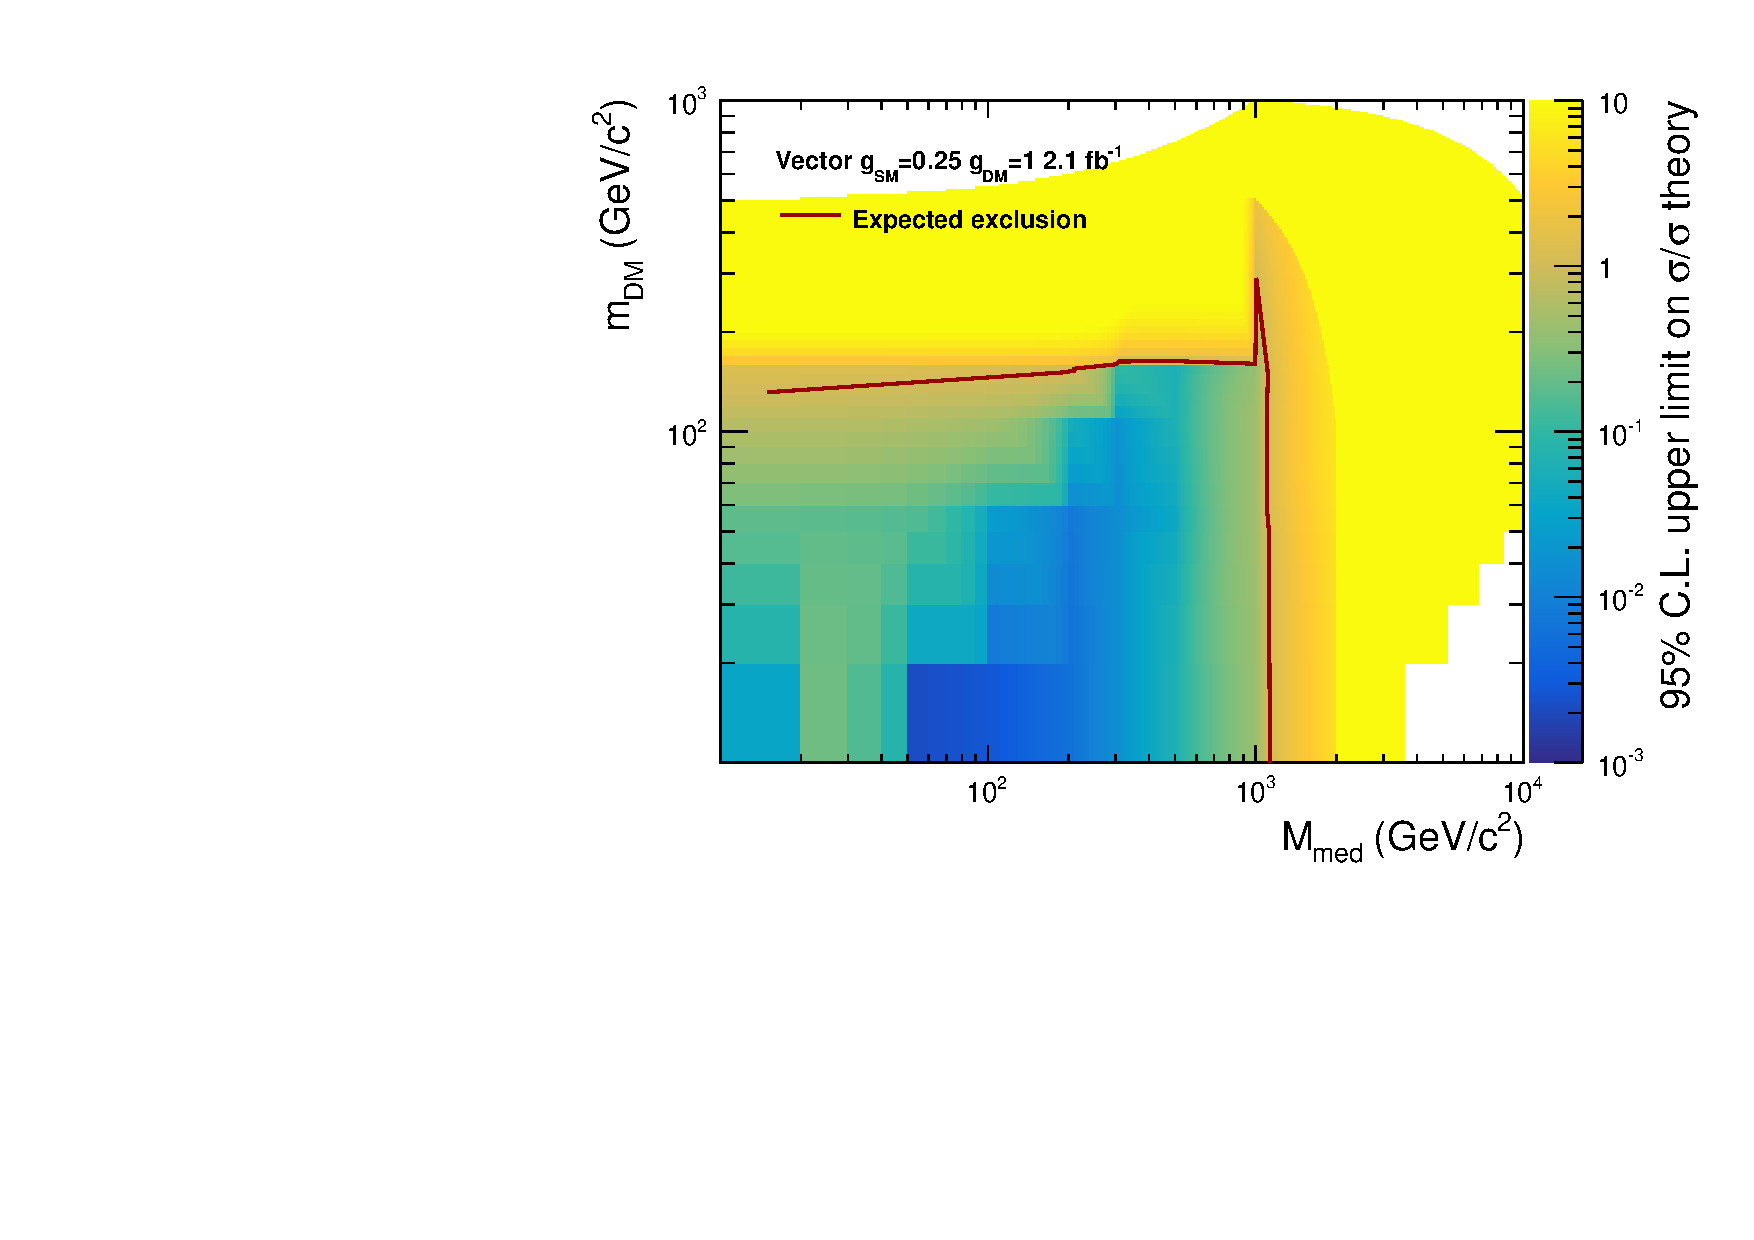
\includegraphics[width=0.75\textwidth]{figures/DMplots/DMV_finalCanvasExpLimit.pdf} \\
\caption{Expected 95\% CL upper limit on the cross section, and exclusion
contour for the vector light flavour model with unity couplings at 2~\ifb.}
\label{fig:dm_A_g1_2fb_2dlimits}
\end{center}
\end{figure}




\begin{figure}
\begin{center}
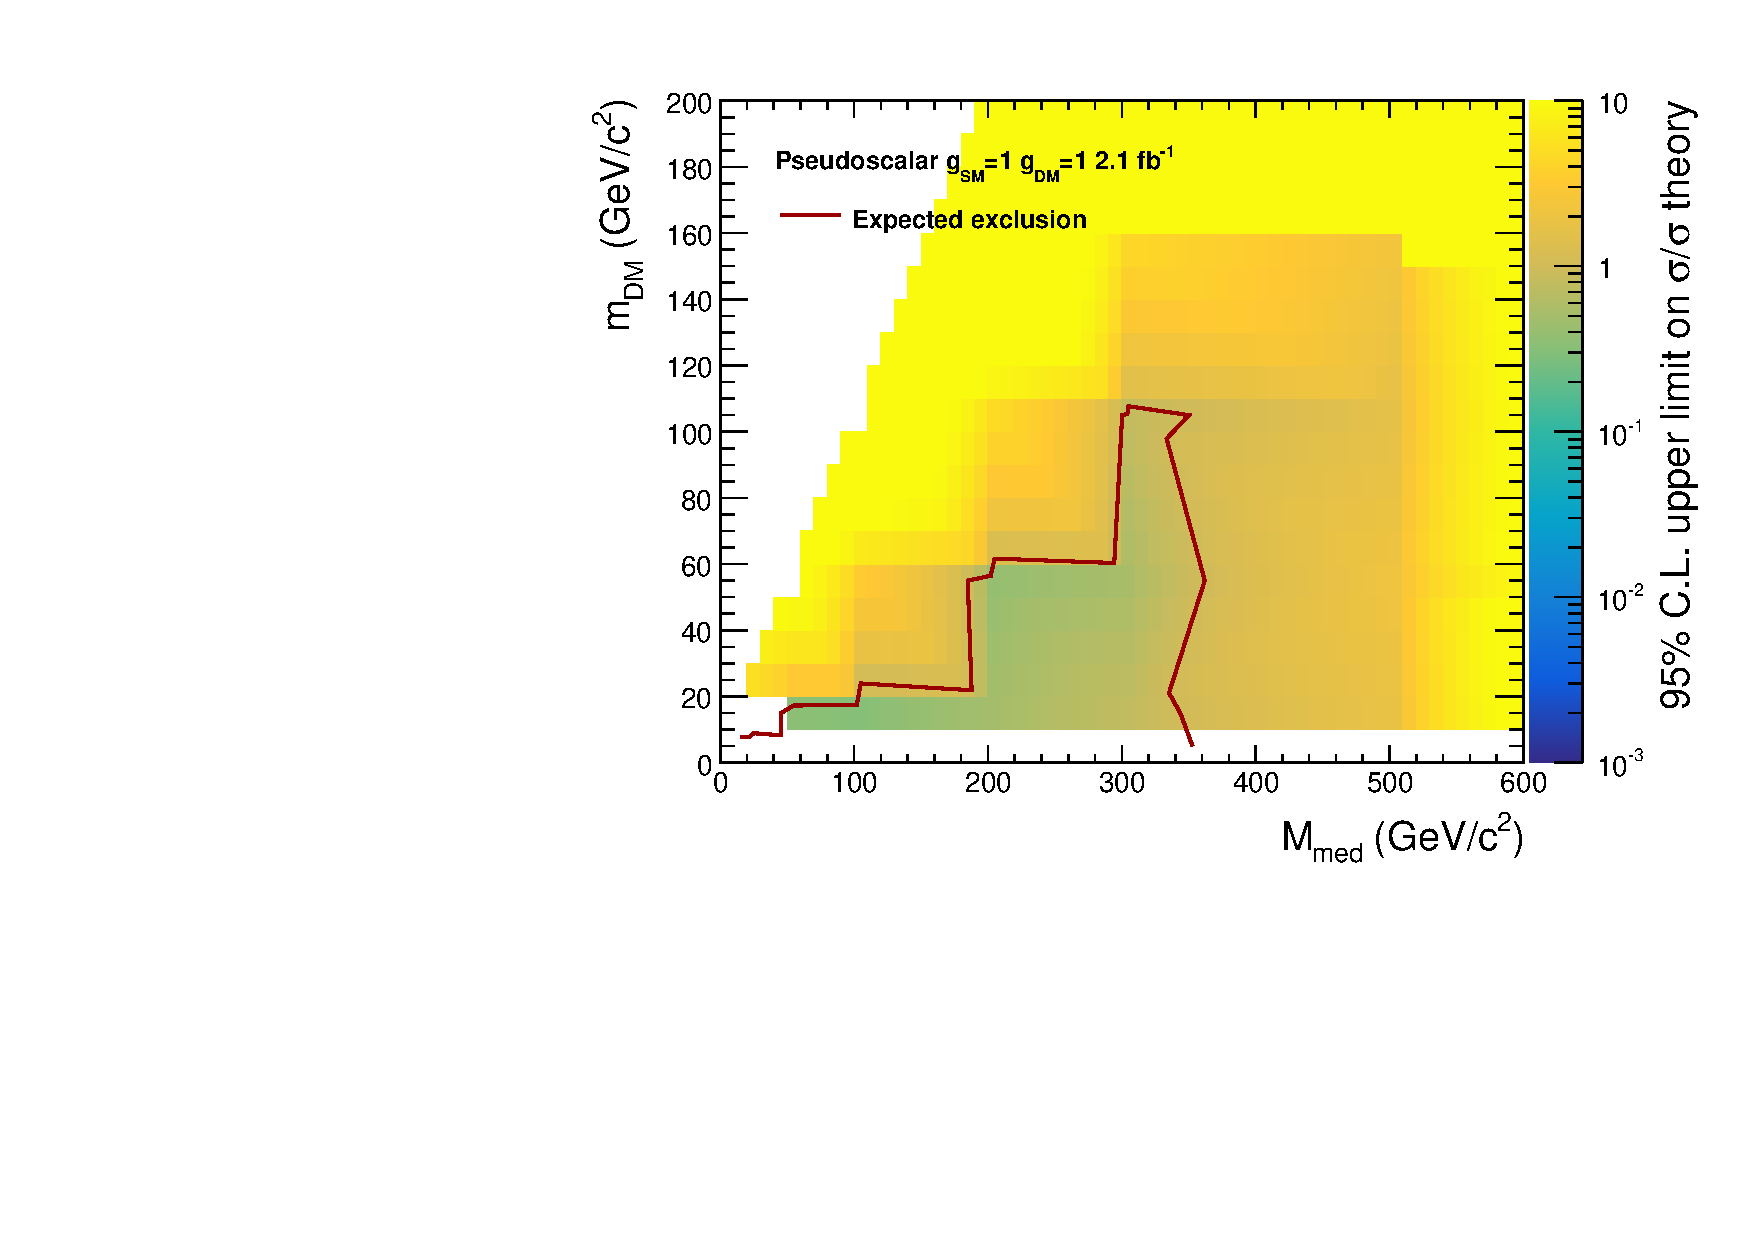
\includegraphics[width=0.75\textwidth]{figures/DMplots/DMP_finalCanvasExpLimit.pdf} \\
\caption{Expected 95\% CL upper limit on the cross section, and exclusion
contour for the pseudoscalar light flavour model with unity couplings at 2~\ifb.}
\label{fig:dm_P_g1_2fb_2dlimits}
\end{center}
\end{figure}


 \subsection{Heavy flavour models} \label{sec:dm_heavyjet}

Owing to the principal of Minimal Flavor Violation (MFV), top and bottom quarks can play important roles in the phenomenology of dark matter. Scalar and
pseudoscalar models predict not only the `monojet' processes described in Sec.~\ref{sec:dm_lightjet} but also the production of dark matter in association
with top (or bottom) pairs. This results in signatures with relatively large jet multiplicities, in particular for \DMtt production. The \alphat analysis is well 
suited to searching for such signatures.  The expected 95\% CL signal strength limits for simplified \DMtt models with scalar and
pseudo-scalar couplings are calculated for 2~\ifb. An uncertainty of 20\% is assumed for all heavy quark samples.
Expected limits obtained for DM+$t\bar{t}$ are given in Tables~\ref{limits_DMttP_xs10_2p1fb_exp}-\ref{limits_DMttS_xs10_2p1fb_exp}.

\begin{table}
\begin{center}
\caption{DMttP xs10 2p1fb exp 95\% CL upper limits}
\begin{tabular}{lcccccccc}
\label{limits_DMttP_xs10_2p1fb_exp}
\multirow{5}{*}{\rotatebox{90}{$m_{\rm{DM}}$ (GeV)}}
& \multicolumn{1}{c|}{500} &  &  &  &  &  &  & 2.83e+04\\ 
& \multicolumn{1}{c|}{150} &  &  &  &  & 509.12 &  & 37.06\\ 
& \multicolumn{1}{c|}{50} &  &  & 116.37 &  & 3.90 & 7.22 & \\ 
& \multicolumn{1}{c|}{10} & 42.02 &  & 2.27 & 2.80 &  &  & \\ 
& \multicolumn{1}{c|}{1} & 1.83 & 2.21 & 2.37 & 2.69 & 4.15 & 5.98 & 35.21\\ 
\cline{2-9}
& \multicolumn{1}{c|}{} & 10 & 20 & 50 & 100 & 200 & 300 & 500\\ 
& & \multicolumn{6}{c}{$M_{\rm{Med}}$ (GeV)}
\end{tabular}
\end{center}
\end{table}


\begin{table}
\begin{center}
\caption{DMttS 2.1\ifb exp 95\% CL upper limits}
\begin{tabular}{lccccccccc}
\label{limits_DMttS_xs10_2p1fb_exp}
\multirow{5}{*}{\rotatebox{90}{$m_{\rm{DM}}$ (GeV)}}
& \multicolumn{1}{c|}{500} &  &  &  &  &  &  & 9.38e+04 & \\ 
& \multicolumn{1}{c|}{150} &  &  &  &  & 1.24e+03 &  & 42.92 & \\ 
& \multicolumn{1}{c|}{50} &  &  & 207.56 &  & 4.29 & 8.25 &  & \\ 
& \multicolumn{1}{c|}{10} & 24.40 &  & 0.89 & 1.97 &  &  &  & \\ 
& \multicolumn{1}{c|}{1} & 0.38 & 0.49 & 0.77 & 2.06 & 4.97 & 8.77 & 34.88 & 304.60\\ 
\cline{2-10}
& \multicolumn{1}{c|}{} & 10 & 20 & 50 & 100 & 200 & 300 & 500 & 1000\\ 
& & \multicolumn{7}{c}{$M_{\rm{Med}}$ (GeV)}
\end{tabular}
\end{center}
\end{table}



The expected 95\% CL signal strength limits for simplified DM+$t(\bar{t})$ models with scalar and pseudo-scalar couplings are calculated for 2~\ifb. An uncertainty of 20\% is assumed for all 
heavy quark samples. 
%Figure~\ref{fig:dm_DMttS_2fb_2dlimits} shows the interpolated scalar expected exclusion contour in the {\mphi-\mchi} mass plane. 
Expected limits obtained for DM+$t\bar{t}$ are given in Tables~\ref{limits_DMbbP_xs10_2p1fb_exp}-\ref{limits_DMbbS_xs10_2p1fb_exp}. 

\begin{table}
\begin{center}
\tiny
\caption{DMbbP xs10 2p1fb exp 95\% CL upper limits}
\begin{tabular}{lccccccccccccc}
\label{limits_DMbbP_xs10_2p1fb_exp}
\multirow{6}{*}{\rotatebox{90}{$m_{\rm{DM}}$ (GeV)}}
& \multicolumn{1}{c|}{1000} & 2.03e+08 &  &  &  &  &  &  &  &  &  &  & 1.44e+08\\ 
& \multicolumn{1}{c|}{500} & 3.76e+06 &  &  &  &  &  &  &  &  & 2.79e+06 & 1.67e+05 & \\ 
& \multicolumn{1}{c|}{150} &  &  &  &  &  &  & 3.14e+04 & 5.07e+03 &  & 3.16e+03 &  & \\ 
& \multicolumn{1}{c|}{50} & 6.87e+03 &  &  & 5.53e+03 & 1.50e+03 &  & 162.84 &  &  &  &  & \\ 
& \multicolumn{1}{c|}{10} & 1.60e+03 & 827.41 &  & 156.65 &  & 105.24 &  &  &  &  &  & \\ 
& \multicolumn{1}{c|}{1} & 177.94 &  & 78.47 & 70.34 &  & 93.38 & 180.58 &  & 415.85 & 2.64e+03 &  & 3.36e+04\\ 
\cline{2-14}
& \multicolumn{1}{c|}{} & 10 & 15 & 20 & 50 & 95 & 100 & 200 & 295 & 300 & 500 & 995 & 1000\\ 
& & \multicolumn{11}{c}{$M_{\rm{Med}}$ (GeV)}
\end{tabular}
\end{center}
\end{table}

\begin{table}
\begin{center}
\tiny
\caption{DMbbS xs10 2p1fb exp 95\% CL upper limits}
\begin{tabular}{lccccccccccccc}
\label{limits_DMbbS_xs10_2p1fb_exp}
\multirow{6}{*}{\rotatebox{90}{$m_{\rm{DM}}$ (GeV)}}
& \multicolumn{1}{c|}{1000} & 1.03e+09 &  &  &  &  &  &  &  &  &  &  & 7.52e+08\\ 
& \multicolumn{1}{c|}{500} & 1.27e+07 &  &  &  &  &  &  &  &  & 1.08e+07 & 1.48e+06 & \\ 
& \multicolumn{1}{c|}{150} &  &  &  &  &  &  & 6.97e+04 & 2.12e+04 &  & 2.72e+03 &  & \\ 
& \multicolumn{1}{c|}{50} & 7.24e+03 &  &  & 5.96e+03 & 2.09e+03 &  &  &  &  &  &  & \\ 
& \multicolumn{1}{c|}{10} & 828.51 & 210.29 &  & 24.07 &  & 43.11 &  &  &  &  &  & \\ 
& \multicolumn{1}{c|}{1} & -1.00 &  & 21.19 & 11.30 &  & 38.25 & 161.04 &  & 290.34 & 1.85e+03 &  & 3.10e+04\\ 
\cline{2-14}
& \multicolumn{1}{c|}{} & 10 & 15 & 20 & 50 & 95 & 100 & 200 & 295 & 300 & 500 & 995 & 1000\\ 
& & \multicolumn{11}{c}{$M_{\rm{Med}}$ (GeV)}
\end{tabular}
\end{center}
\end{table}



\clearpage
